% !TEX encoding = UTF-8
% !TEX TS-program = pdflatex
% !TEX root = ../tesi.tex

%**************************************************************
\chapter{Comparisons of the solutions}
\label{cap:comparisons}
%**************************************************************

\intro{Here all the observations detected while using Typecript and Scala for our case study will be presented}\\

%**************************************************************
\section{Code readability in TypeScript vs in Scala}

\subsection{Readability in TypeScript}
TypeScript's programs have a really readable code.
In the implementation we can appreciate how the passing of the builders methods' parameters have been achieved in a concise way using the JSON format.
This is fitting very well in a declarative approach, granting compact code solutions. 
On the other hand, some shortcomings of the language caused the code to lose part of the readability and conciseness.\\
\subsubsection{Less readable code with pulumi.all and .apply}
\label{sssec:ts-subnets-comparison}
Lets consider once again the TypeScript version of the function that is responsible for creating the subnets across the various availability zones:\\
\begin{minipage}{\linewidth}
  \begin{lstlisting}[numbers=left, numberstyle=\tiny, numbersep=-5pt, stepnumber=1, linewidth=420pt]
    protected createAZsSubnets(isPvt: Boolean) : Output<Subnet[]>{
      this.availableZones = aws.getAvailabilityZonesOutput()
      return pulumi.all([this.availableZones.names, this.vpc!.id]).apply(([azNames, vpcId]) => {
        let i = 0
        let listToPushInto: Subnet[] = Array<aws.ec2.Subnet>()
        azNames.forEach(azName => {
          let fullName = azName + (isPvt ? "-pvt" : "-pub") + "-subnet-typescript"
          listToPushInto.push(new Subnet(fullName, {
            vpcId: vpcId,
            availabilityZone: azName,
            cidrBlock: isPvt ? this.pvtSubnetsCidrs[i] : this.pubSubnetsCidrs[i],
            tags: {
              Name: fullName,
            },
          },{
            parent: this.vpc
          }));
          i++;
        });
        return listToPushInto
      });
    }
  \end{lstlisting}
  \end{minipage}
%\begin{center}
%  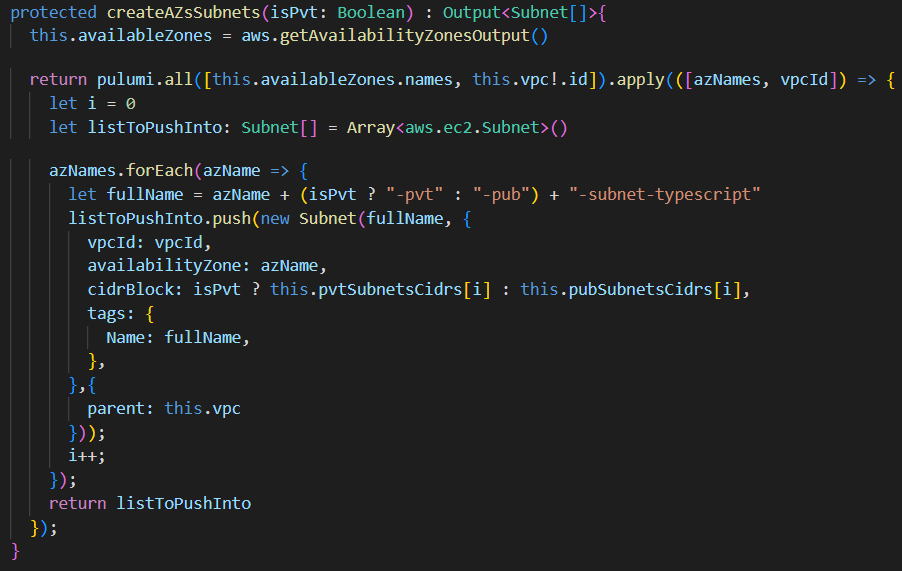
\includegraphics[width=1.0\columnwidth]{comparisons/ts_create_subnets} 
%  \captionof{figure}{TypeScript subnets creation}
%\end{center}\mbox{}\\
When talking about readability, the \texttt{pulumi.all} and the \texttt{apply} functions are quite cryptic.
It takes us a little time to understand what are the return types of the \texttt{pulumi.all} and of the \texttt{apply} functions.
I remind here that the types of these two functions are fully explained in the \hyperref[par:ts-lambda]{The apply's lambda} paragraph.\\
We'll make further considerations on this function in the \hyperref[sssec:readability-for-yield]{Readability of the Scala's for-yield vs pulumi.all and .apply} paragraph.

\subsection{Readability in Scala}
Scala is in general more verbose than TypeScript, but the extreme flexibility of the language let us define a powerful \textit{syntactic sugar} that allowed for a even more readable and concise solution compared to the TypeScript one.
The combination of the various features, among which we can find currying, \texttt{using} and \texttt{given} keywords, and the monads, grant Scala the possibility to define \gls{internal DSL}s.
Thanks to this characteristic, also in Scala I achieved a surprisingly readable code while defining the resources to be created on our Pulumi \textit{stack}.

\subsubsection{Function currying}
The currying of Scala used to define our \textit{sugared} functions granted us the possibility to declare the resources with this syntax:
\begin{verbatim}
  val resourceName = sugaredResourceConstructor("res-name") {
    firstParameter(...)
    secondParameter(...)
    ...
  }
\end{verbatim}\mbox{}\\
This code is really readable (it resembles to a function definition) and is perfectly fitting in a declarative approach since we can have a straight list of the parameters we want to set for our resource.\\

\subsubsection{Hidden builders}
Thanks to the \texttt{given} and \texttt{using} keywords, builders aren't manually instantiated and we don't require to explicitly say on which builder instance we are calling the builders' methods.
This is letting us have an even more lightweight code that is really just focusing on \textit{what} we need to instantiate instead of \textit{how} we could instantiate it.
Let's consider the VPC creation in our Scala solution and how would it be created instead in a Java solution.\\
Scala solution:\\
\begin{minipage}{\linewidth}
\begin{lstlisting}[numbers=left, numberstyle=\tiny, numbersep=-5pt, stepnumber=1]
  val myVpc = vpc("scala-main") {
    cidrBlock("10.136.0.0/24")
    tags("Name" -> "myVpcScala")
  }
\end{lstlisting}
\end{minipage}
Java solution:\\
\begin{minipage}{\linewidth}
\begin{lstlisting}[numbers=left, numberstyle=\tiny, numbersep=-5pt, stepnumber=1]
  protected Vpc vpc = new Vpc("my-vpc-java", VpcArgs.builder()
    .cidrBlock("10.136.0.0/24")
    .instanceTenancy("default")
    .tags(Map.of("Name", "myVpcJava"))
    .build(),
          CustomResourceOptions.builder()
                  .parent(this)
                  .build());
\end{lstlisting}
\end{minipage}
Even if our \textit{syntactic sugar} is using the very same APIs used from the Java's solution, the readability and the conciseness are entirely on another level.

\subsubsection{Implicit conversion functions to get rid of Map and List constructors while passing a single value}
The implicit conversion functions presented in the \hyperref[sssec:implicit-converion-functions]{Implicit conversion functions} paragraph let us get rid of the constructor of the \texttt{Map} and of the \texttt{List} if we're interested in passing a single value.\\
It is common, while declaring a new resource, to pass a single parameter to a builder's method that is, in truth, expecting a \texttt{List} or a \texttt{Map} parameter.
In such cases syntax at line 3 of the following block of code could be annoying:\\
\begin{minipage}{\linewidth}
  \begin{lstlisting}[numbers=left, numberstyle=\tiny, numbersep=-5pt, stepnumber=1]
    val myVpc = vpc("scala-main") ({
        cidrBlock("10.136.0.0/24")
        tags(Map("Name" -> "myVpcScala"))
      },{
        parent(this)
      })
  \end{lstlisting}
  \end{minipage}
%\begin{center}
%  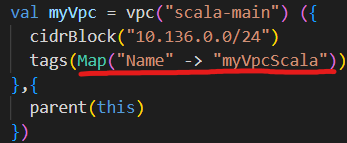
\includegraphics[width=0.7\columnwidth]{comparisons/explicit_map} 
%  \captionof{figure}{Singleton map for a parameter}
%\end{center}\mbox{}\\
%Tags expects a \texttt{Map[String, String]} value, but if we want to pass a single map element, we would appreaciate to get rid of the Map constructor and just write \texttt{"Name -> "myVpcScala"}.
But thanks to the implicit conversion functions the final result, as we have seen, is the desired one:\\
\begin{minipage}{\linewidth}
  \begin{lstlisting}[numbers=left, numberstyle=\tiny, numbersep=-5pt, stepnumber=1]
    val myVpc = vpc("scala-main") ({
        cidrBlock("10.136.0.0/24")
        tags("Name" -> "myVpcScala")
      },{
        parent(this)
      })
  \end{lstlisting}
  \end{minipage}
%\begin{center}
%  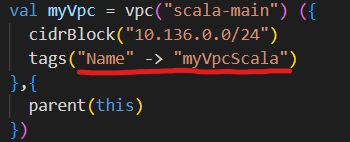
\includegraphics[width=0.7\columnwidth]{comparisons/implicit_map} 
%  \captionof{figure}{Tuple for a parameter}
%\end{center}\mbox{}\\
For a single parameter the difference of effort in explicitly writing the \texttt{Map} constructor can be negligible, but when it comes to define many resources that use multiple methods that accept collections as input parameters, such a feature can really save us a lot of keystrokes, while keeping our code more readable and simple.

\subsubsection{Readability of the Scala's for yield vs pulumi.all and apply}
\label{sssec:readability-for-yield}
Lets consider the function that creates the subnets.
With respect to the TypeScript solution, the Scala one is more readable:\\
\begin{minipage}{\linewidth}
  \begin{lstlisting}[numbers=left, numberstyle=\tiny, numbersep=-5pt, stepnumber=1]
  def createAzSubnets(isPvt: Boolean) =
    for
      azRes <- availabilityZonesNames()
      myVpcId <- myVpc.id()
      tuples = azRes.names().zip(if isPvt then pvtSubnetsCidrs else pubSubnetsCidrs)
    yield
      tuples.map((name, cidr) => {
        val fullName = name + "-" + (if isPvt then "pvt" else "pub") + "-subnet-scala"
        subnet(fullName) ({
          vpcId(myVpcId)
          availabilityZone(name)
          cidrBlock(cidr)
          tags("Name" -> fullName)
        },{
          parent(myVpc)
        })
    })
  \end{lstlisting}
\end{minipage}
%\begin{center}
%  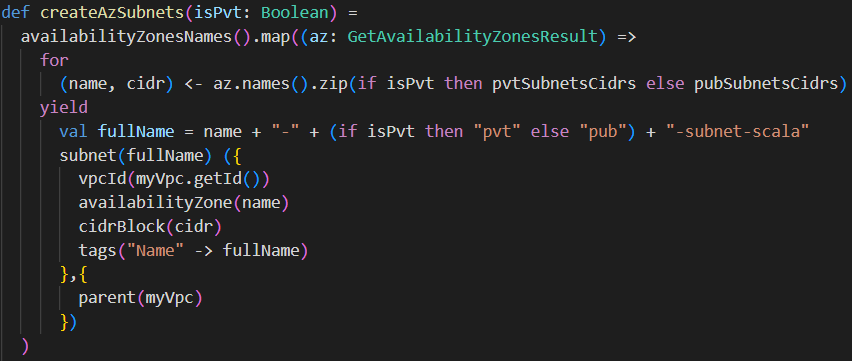
\includegraphics[width=1.0\columnwidth]{comparisons/scala_create_subnets} 
%  \captionof{figure}{Scala subnets creation}
%\end{center}\mbox{}\\
All the logic to \textit{unbox} the \texttt{Output} values in order to execute some operations on them is neatly hidden behind the transparent monadic implementation of the \texttt{Output} type.
This enables a more elegant and concise solution based just on well known constructs such as the for loop and the map function.
This allowed to get rid of the cryptic \texttt{pulumi.all} function and let us successfully hid the \texttt{apply} function in the monadic implementation, without requiring the user to explicitly use it.\\
TypeScript needed for us to rely on the \texttt{pulumi.all} function in order to craft a single \texttt{Output} value out of two, so that the \texttt{apply} function, that is capable to work on a single \texttt{Output} value, could be used to get the work done.\\
Here instead we are separately \textit{unboxing} the \texttt{Output} values with the combination of the expressiveness of the Scala for yield's enumerators and the \textit{unboxing} operation granted by the \texttt{Output[Monad]}.\\
%First, the \texttt{map} function is much more intuitive with respect to the \texttt{pulumi.all} and \texttt{apply} combination in the \hyperref[sssec:ts-subnets-comparison]{TypeScript implementation}.
%Moreover, the for comprehension used in the Scala version is a more elegant and concise solution.
%In fact, the map function is doing the work of both the \texttt{pulumi.all} and \texttt{apply} functions, with much less code and in a much more readable way.\\
%Furthermore, with Scala we're using the language feature of the for comprehension to automatically create a collection of the generated subnets and return them all together.\\
Furthermore, TypeScript implementation requires us to explicitly insert the generated subnets in a variable as a side effect of the \texttt{foreach}, while Scala is automatically achieving it with the for yield construct.\\
Always in TypeScript, we also have to explicitly return the list at the end of the \texttt{apply}'s lambda, that would otherwise return an \texttt{Output<void>} value.\\
All this is making the TypeScript solution for the subnets creation much more cumbersome than the Scala counterpart.


\section{Expressiveness in TypeScript vs in Scala}
Are here better expressed the observations made during the \hyperref[sssec:readability-for-yield]{Readability of the Scala's for yield vs pulumi.all and .apply} paragraph.

\subsection{pulumi.all and .apply vs for comprehension and monads}

\subsubsection{TypeScript compensate for its lack of expressiveness with the pulumi.all function}
In the \hyperref[sssec:pulumi-all]{pulumi.all} paragraph of the subnets creation section, we have seen how the concatenation of \texttt{apply} to the \texttt{pulumi.all} function let us create the subnets across the various availability zones.
Anyway, The process of wrapping two different \texttt{Ouptut} values in a single \texttt{Output} using the \texttt{pulumi.all} function, and then extract that newly created value form the \texttt{Output} \textit{context} is verbose and complex.\\
The \texttt{pulumi.all} function is effective but its existence is required to compensate for the lack of expressiveness of the TypeScript language.

\subsubsection{Scala's expressiveness let us get rid of pulumi.all}
The functional nature of the Scala language let us get rid of the \texttt{pulumi.all} function thanks to the monad implementation for the \texttt{Output} type.
The for yield, exploting the monadic type of \texttt{Output}, is letting us \textit{unbox} the single \texttt{Output}s separately, in a flexible and intuitive way.\\
Furthermore, the \texttt{apply} function that we had to explicitly invoke in the TypeScript solution, became in Scala the actual implementation of the \texttt{flatMap} function for the \texttt{Output[Monad]}, being totally invisible to the user.
%The \texttt{map} function that we used in our function for the \hyperref[sssec:subnets-creation]{subnets creation} has been implemented only on the bases of the \texttt{flatMap} function.
%So, we replaced the \texttt{pulumi.all} function with the \texttt{map} function offered by the \texttt{Monad[Output]}, and the \texttt{apply} function is now hidden behind the \texttt{map} implementation.\\
This achievement is perfectly depicting how the expressiveness of Scala permitted us to satisfy our need of applying functions on multiple separated \texttt{Output} values without resorting to an ad-hoc function created only for that specific purpose (\texttt{pulumi.all}).
In fact, we would be able to implement a monad for any \textit{context} type, while \texttt{pulumi.all} is working exclusively with the \texttt{Output} type.
Moreover, the for loop is is much more intuitive to an user rather than the \texttt{pulumi.all} and the explicit \texttt{apply} functions combination.

%On the other hand, when we have to combine two values of different \texttt{Output}s types in another value of another \texttt{Output} type, we must rely on the \texttt{pulumi.all} and \texttt{.apply} functions.
%In the \hyperref[sssec:pulumi-all]{pulumi.all} paragraph we have seen how such a function is used in the TypeScript implementation to create the subnets in our availability zones.


%Now, if we want to use the \texttt{.apply} function to 
%since we have to pass through a pulumi.all to wrap the availability zones names \texttt{Output<String[]>} and the 


%\subsubsection{Poor tools to act on groups of Outputs}

%\section{Java solution observations}

%\subsection{Advantages of using Pulumi's Java APIs}

%\subsection{Disadvantages of using Pulumi's Java APIs}

%\subsubsection{Verbose code}

%\section{My Scala solution observations}

%\subsection{Advantages of using my Scala \textit{syntactic sugar}}

%\subsubsection{Very concise code}

%\subsubsection{Very readable and elegant code}

%\subsubsection{More powerful constructs thanks to the for-comprehension and the monads to act on groups of Outputs}

%\subsection{Disadvantages of using my Scala \textit{syntactic sugar}}

%\subsubsection{Partial solution, not all the corner cases have been considered}

%\section{Final thoughts on the Scala solution}